\section{Windows}

Officially, the pbdR team does not support gaming consoles.  However, it is possible to install pbdR packages on Windows.

\subsection{R and Rtools}

The instructions and screenshots for this document are for version 2.15.1 of R, but later versions should be very similar, if not identical.






\subsubsection{R}


\begin{enumerate}
  \item Download R: \url{http://cran.r-project.org/bin/windows/base/} \label{enum:windl}
  \sshots{\begin{center}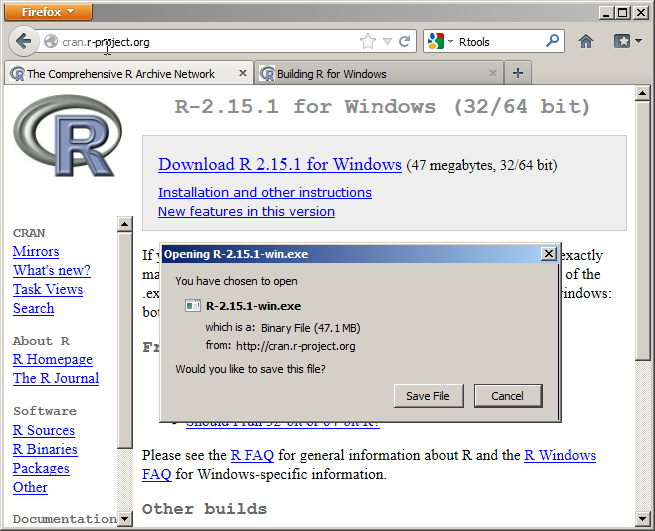
\includegraphics[scale=.5]{windows/pics/R_1.png}\end{center}}
  %
  \item Open the saved file from \ref{enum:windl} above to begin the installation.  At the first setup screen, click 'Next' to continue.
  \sshot{windows/pics/R_2.png}
  %
  \item When prompted with the license, click 'Next' to continue.
  \sshot{windows/pics/R_3.png}
  %
  \item When prompted for the location to install R, we strongly encourage you to use the default.  When you have made your decision, click 'Next'.
  \sshot{windows/pics/R_4.png}
    %
  \item When prompted with the components to install, you should select a 'User installation'.  Then click 'Next'.
  \sshot{windows/pics/R_5.png}
    %
  \item When prompted with the option to alter the startup options, we suggest selecting \code{No (accept defaults)}.  When you have made your decision, click 'Next'.
  \sshot{windows/pics/R_6.png}
    %
  \item When prompted with the start menu folder options, make your choice and then click 'Next'.
  \sshot{windows/pics/R_7.png}
    %
  \item When prompted with the additional tasks options, we suggest making sure that \code{Save version number in registry} and \code{Associate R with .RData files} are both \textbf{checked}.  When you have made your decisions, click 'Next'.
  \sshot{windows/pics/R_8.png}
  %
  \item To complete the R installation, select 'Finish'.
  \sshot{windows/pics/R_9.png}
  %
\end{enumerate}





\subsubsection{Rtools}

\begin{enumerate}
  \item Download Rtools: \url{http://cran.r-project.org/bin/windows/base/} \label{enum:rtoolsdl}
  \sshots{\begin{center}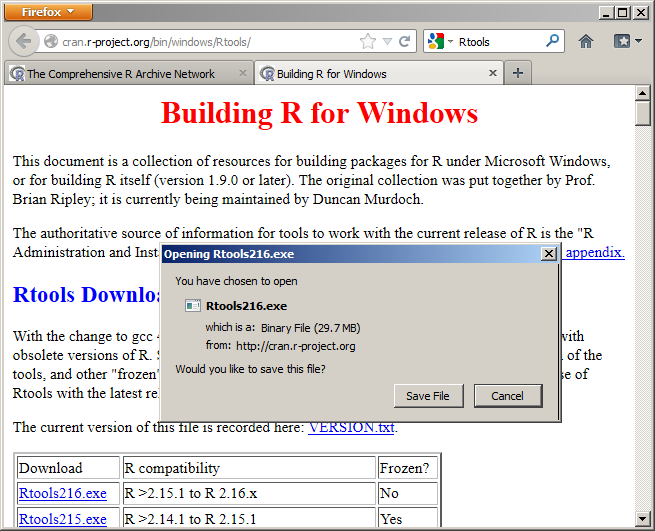
\includegraphics[scale=.5]{windows/pics/Rtools_1.png}\end{center}}
  %
  \item Open the saved file from \ref{enum:rtoolsdl} above to begin the installation.  At the first setup screen, click 'Next' to continue.
  \sshot{windows/pics/Rtools_2.png}
  %
  \item When prompted with the license, click 'Next' to continue.
  \sshot{windows/pics/Rtools_3.png}
  %
  \item When prompted for the location to install R, we strongly encourage you to use the default.  When you have made your decision, click 'Next'.
  \sshot{windows/pics/Rtools_4.png}
    %
  \item When prompted with the components to install, you should select a 'User installation'.  Then click 'Next'.
  \sshot{windows/pics/Rtools_5.png}
    %
  \item When prompted with the option to alter the startup options, we suggest selecting \code{No (accept defaults)}.  When you have made your decision, click 'Next'.
  \sshot{windows/pics/Rtools_6.png}
    %
  \item When prompted with the start menu folder options, make your choice and then click 'Next'.
  \sshot{windows/pics/Rtools_7.png}
    %
  \item To complete the Rtools installation, select 'Finish'.
  \sshot{windows/pics/Rtools_8.png}
  %
\end{enumerate}
